%Edit 0036 ZZZ to report number nnnn 
%Edit 2.7.1 YYMILE to milestone number m.m.m
%Edit Identification of suitable preconditioner techniques YYTITLE to report title - Words Start with Caps
\documentclass[11pt,twoside,a4paper]{article}
%%======================================================================
%% PACKAGES:
%%
%\usepackage{times}               % Times+Helvetica+Courier fonts
\usepackage{helvet}              % helvetica + cmr
\usepackage{fancyhdr}       % package for headers/footers
\usepackage{amsmath}
\usepackage{amssymb}
\usepackage{graphicx}            % Graphics.
%\usepackage{a4}                  % page layout to fit A4
%\usepackage{lastpage}            % get page no of last page
%\usepackage{ifthen}              % logical branching
\usepackage{hyperref}            %insert hyper-links
\usepackage{latexsym}
% uncomment the following to override auto page total
%\pptotal{20}
%%======================================================================

% ensure sans-serif font used throughout
\renewcommand{\familydefault}{\sfdefault}

\newcommand{\culhamissueno}{1.00}%<==edit
\newcommand{\culhamshorttitle}{CD/EXCALIBUR-FMS/0036}%<==edit
\newcommand{\Sec}[1]{Section~\ref{sec:#1}}
\newcommand{\Fig}[1]{Figure~\ref{fig:#1}}
\newcommand{\Tab}[1]{Table~\ref{tab:#1}}
\newcommand{\Eq}[1]{Equation~(\ref{eq:#1})}
\newcommand{\Eqs}[2]{Equations(\ref{eq:#1}) and~(\ref{eq:#2})}
\newcommand{\Figs}[2]{Figures~\ref{fig:#1}--~\ref{fig:#2}}
%Bold lc for script names, tt for computer code and file-names
%\F{NEPTUNE} always in caps
\newcommand{\F}[1]{\textsc{#1}}
\newcommand{\B}[1]{\textbf{#1}}
\newcommand{\T}[1]{{\tt #1}}
\newcommand{\V}[1]{\mathbf{#1}}
\newcommand{\I}[1]{\textit{#1}}
\newcommand{\nep}{\textsc{NEPTUNE}}
\newcommand{\exc}{\textsc{E}x\textsc{CALIBUR}}
\newcommand{\Papp}{Proxyapp}
\newcommand{\papp}{proxyapp}



%%======================================================================

%% REPORT COVER PAGE Information

\newcommand{\culhamtitle}{\LARGE Identification of suitable preconditioner techniques  \\[1.0\baselineskip] M2.7.1 }%<==edit

%%QA BOX information -- change following as needed
\newcommand{\culhamboardname}{Martin O'Brien}%<==edit
\newcommand{\culhamcontactname}{Rob Akers}%<==edit
\newcommand{\culhamauthor}{Wayne Arter}%<==edit
\newcommand{\culhamauthora}{Ed Threlfall}%<==edit
\newcommand{\culhamauthorb}{Joseph Parker}%<==edit
\newcommand{\culhamauthorc}{Will Saunders}%<==edit
%\newcommand{\culhamcontacttel}{Telephone: 01235 466498}
%\newcommand{\culhamcontactemail}{Email: rob.akers@ukaea.uk}

\newcommand{\culhamdate}{\today}%<=edit
\newcommand{\culhamdatea}{\today}%<=edit
\newcommand{\culhamdateb}{\today}%<=edit

% reproduce Rob's page size

\setlength{\textheight}{220.0mm}
\setlength{\textwidth}{165.0mm}
\setlength{\topmargin}{0.0mm}
\setlength{\oddsidemargin}{0.0mm}
\setlength{\evensidemargin}{\oddsidemargin}
\setlength{\parindent}{0mm}
\addtolength{\parskip}{0.5\baselineskip}
\setlength{\topsep}{0pt}
\setlength{\itemsep}{0pt}

%%======================================================================
\begin{document}

%Titlepage comes out wrong size, but should look right apart from
% picture which cannot be wider than c.150mm.
% To produce conforming report rp1pub.pdf
% remove title page by commenting out lines ending in %<==omit, then
% sed -e '/<==omit$/s/^/%/' < rp1.tex > rp1omit.tex
% pdflatex rp1omit;bibtex rp1omit; pdflatex rp1omit
% pdfunite cover.pdf rp1omit.pdf rp1pub.pdf 
\begin{titlepage}%<==omit
\vspace*{-30mm}%<==omit

\includegraphics[width=2.5cm]{../corpics/cofaplus} \\[2.0\baselineskip]%<==omit
{\LARGE {\textbf{\textsf{ExCALIBUR}}}}\\[2.0\baselineskip]%<==omit
{\LARGE \culhamtitle } \\[2.0\baselineskip]%<==omit
{\textbf{\textsf{Abstract}}}\\%<==omit
The report describes work for \exc \ project \nep \ %<==omit
at Milestone 2.7.1. %<==omit
Report on the status of programming models and code generators for the
various node architectures focused on performance, usability, maintainability
and  availability.  
%<==omit
%<==omit
\vfill%<==omit
\centerline{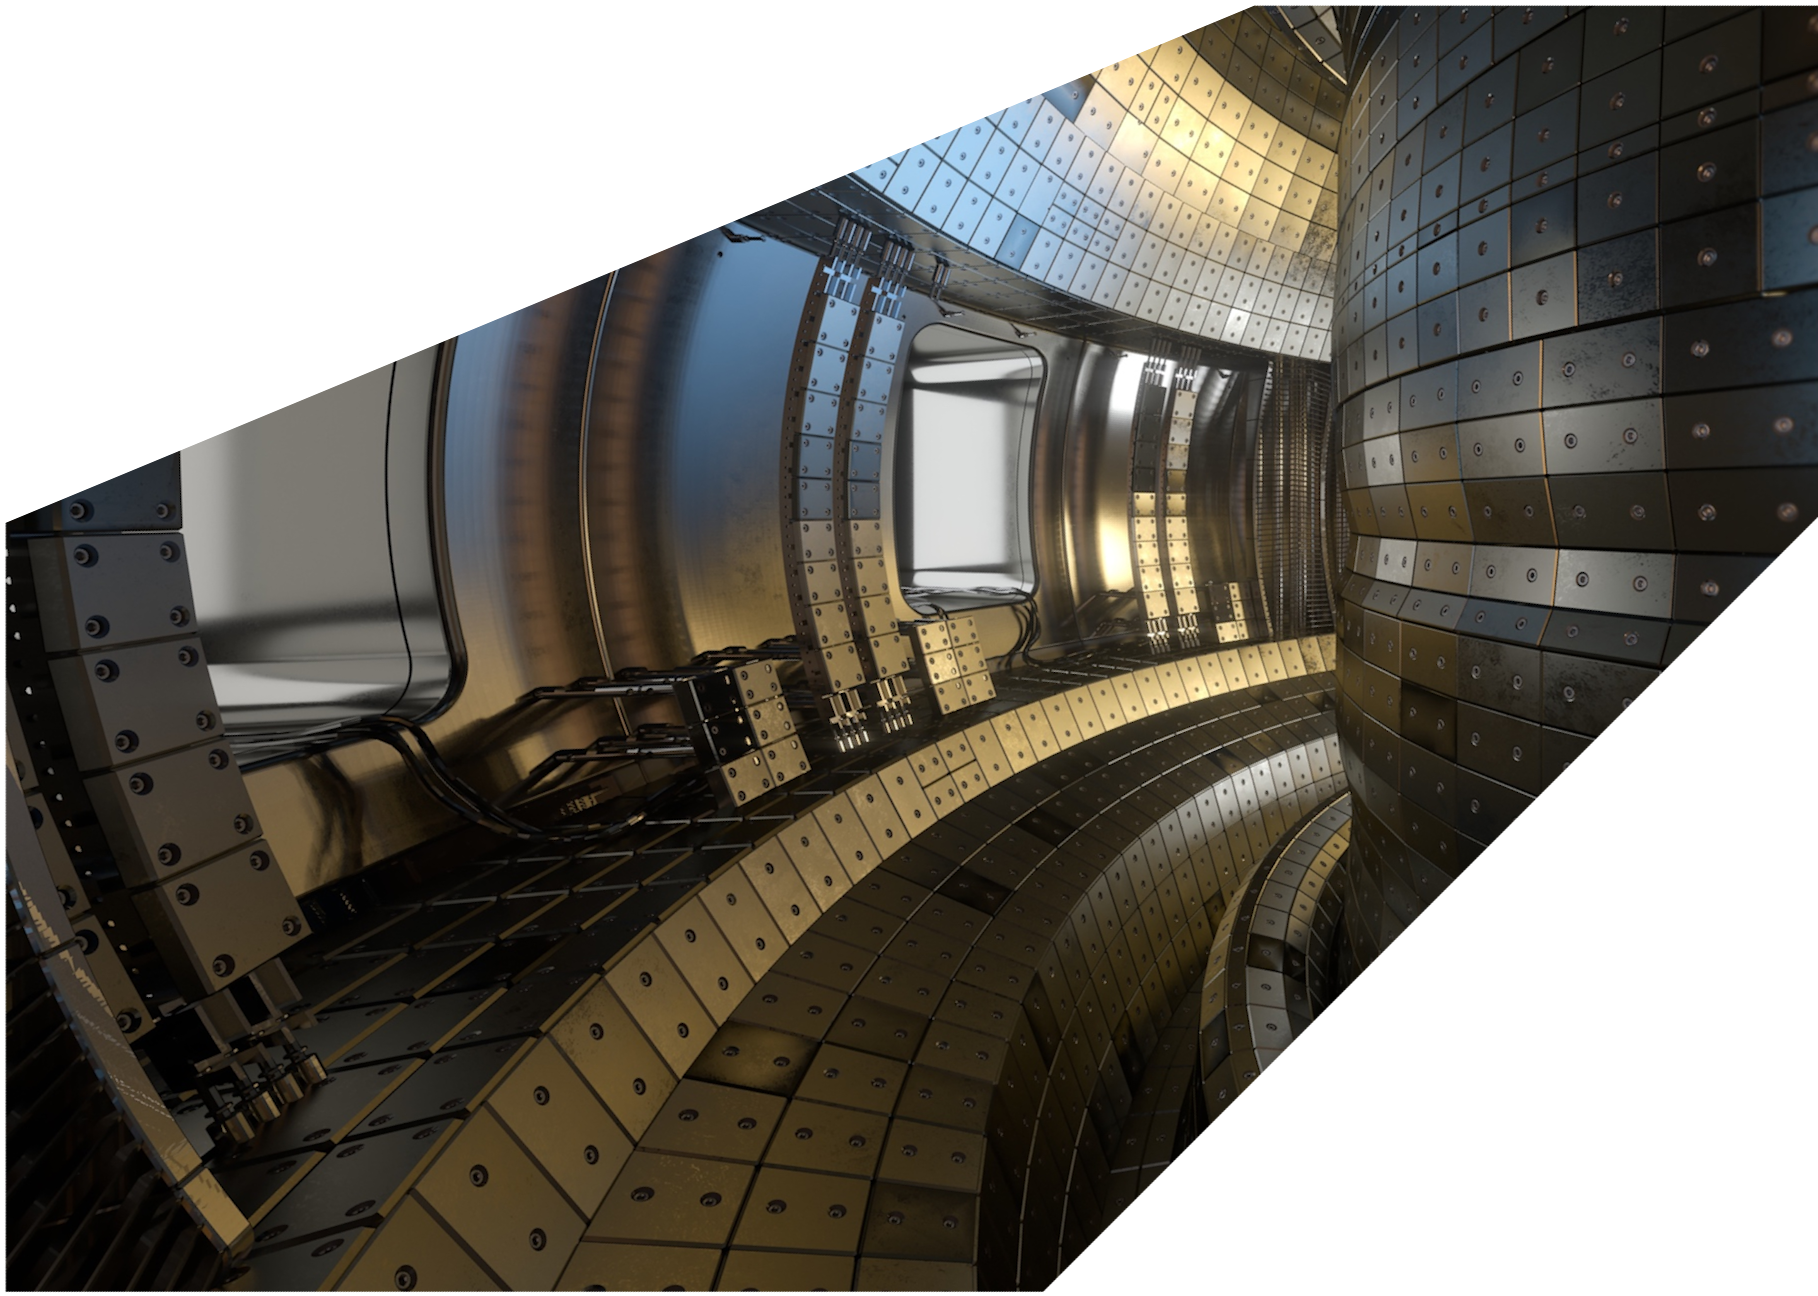
\includegraphics[width=0.9\textwidth]{../corpics/tokintcrop}}%<==omit
\end{titlepage}%<==omit

\hspace{-30mm}\begin{table}[h]
\sffamily
\begin{center}
\textbf{\textsf{UKAEA REFERENCE AND APPROVAL SHEET}}
\begin{tabular}{||p{5.7cm}|p{4.7cm}|p{5.0cm}||}
\hline
\hline
& Client Reference: &  \\
\hline
& UKAEA Reference: & \culhamshorttitle \\
& & \\
\hline
& Issue: & \culhamissueno \\
\hline
& Date: & \culhamdateb \\
\hline
\multicolumn{3}{||l||}{} \\
\multicolumn{3}{||l||}{Project Name: ExCALIBUR Fusion Modelling System} \\
\multicolumn{3}{||l||}{} \\
\hline
\end{tabular}
\begin{tabular}{||p{3.3cm}|p{4.6cm}|p{3.5cm}|p{3.6cm}||}
\hline
& Name and Department & Signature & Date \\
\hline
Prepared By: & \culhamauthora & N/A & \culhamdate \\
& \culhamauthorb & N/A & \culhamdate \\
& \culhamauthorc & N/A & \culhamdate \\
& \culhamauthor & N/A & \culhamdate \\
& & & \\
& BD & & \\
\hline
Reviewed By: & \culhamcontactname & 
\includegraphics[width=3.0cm]{../corpics/blanksign}& \culhamdatea \\
& & & \\
& Advanced Computing Dept. Manager & & \\
\hline
Approved By: & \culhamcontactname  & 
\includegraphics[width=3.0cm]{../corpics/blanksign} & \culhamdateb \\
& & & \\
& Advanced Computing Dept. Manager  & &\\
\hline
\hline
\end{tabular}
\end{center}
\end{table}


\clearpage

\section{{\nep\  Meeting: 22 April 2021 10.15-10.45am BST}}

\emph{Present}

\begin{itemize}
\item Chair: Wayne Arter, UKAEA
\item Ed Threlfall, UKAEA
\item Vassil Alexandrov, STFC
\item Sue Thorne, STFC

\end{itemize}

\section{Minutes}

WA presented the agenda: to go through the most recent report received from STFC, to 
discuss STFC's work since the submission of that report, and to conclude with a 
general discussion about proposed work going forward. The `01'~report~\cite{2047353-TN-01}
was not discussed.

WA thanked ST and VA for their most recent `02' report~\cite{2047353-TN-02}, noting that this 
meeting included only two of the four authors named on the report.  WA praised 
the report as a useful introduction, then noted that it was useful to have 
received also the \LaTeX\ source which allows UKAEA to make minor notational 
corrections.  WA had a slight issue with some of the syntax in the report, 
taken from a textbook to which he had no access (something like 
$diag(\mathcal{L}_x \left ( \phi \right ))$, with the confusion being that the 
diagonal of the matrix would be zero for a centred-difference scheme.  However, 
WA requested no changes to the report.  Another question WA had concerned 
S.3.4, which mentioned other libraries of interest but which did not include 
direct sparse solvers.  ST answered that this section was concerned only with 
preconditioners and iterative methods - not direct solvers.  WA said he was not 
very familiar with direct solver libraries and asked whether ST was proposing 
to use them as part of a preconditioner; ST replied that she was not, but noted 
that direct solvers could be applied to preconditioner sub-blocks (note Jack 
Dongarra list {\it does} include direct solvers); though indicated that the 
sub-blocks are probably too large for direct methods to be useful.  WA 
concurred - he had expected this to the the case - though noted that there was 
historically a commercial direct-solver electromagnetism code (and cited the 
then-lack of understanding of preconditioners for the high-frequency Helmholtz 
problem).  ST noted that \F{MUMPS} can be used directly or for preconditioning 
(incomplete factorization).  WA concluded this discussion by again commending 
the report.

WA moved on to a discussion of work performed since the submission of the 
report; ST confirmed that work had continued.  WA asked whether STFC planned to 
consider stochastic/Monte Carlo methods; ST and VA replied in the 
affirmative.  ST described current work as having two phases: 
\begin{enumerate}
\item Examining integration of preconditioners with \F{BOUT++} and \F{Nektar++} (Emre Sahin has been 
in contact with David Moxey re. the latter code, though this work has been 
delayed by unavoidable circumstance); the aim is to interface a MCMCMI (Markov 
Chain Monte Carlo Matrix Inversion) preconditioner acting on the entire matrix; 
and
\item  work on blocking, for which ST has developed new theory for a class of 
`non-symmetric constraint preconditioners' (her term) aimed at clustering 
eigenvalues, also trying different families of block factorizations for 
efficient generation of preconditioners.  ST is currently working on narrowing 
down the factorizations to the most useful ones. 
\end{enumerate}
WA acknowledged the challenge 
of the problem including hyperbolics, than agreed that the direction of current 
work was promising.

WA asked whether there was anything else to discuss - ST and VA explained that 
their co-workers Anton Lebedev and Emre Sahin were stuck on other projects, so they intend to 
onboard a new person formerly of Manchester and prior to that Jack Dongarra's 
group (and who has worked with Anton/Emre in the past).  WA acknowledged that 
the shortness of this project was a potential issue and also that the 
Manchester group was very strong (and that UKAEA had tried to entice them onto 
\nep\ , though there will be future opportunity to do so).  ST noted the 
advantage of having a flexible team of people at the Hartree Centre.

WA steered the discussion to work going forward.  ST is working on interfaces 
for \F{BOUT++} and \F{Nektar++} and implementing preconditioning for the core 
test problems supplied by Ben Dudson.  ST plans also to test multigrid methods 
against stochastic / Monte Carlo.  WA confirmed that it was acceptable for STFC 
to abandon any directions they judged to be of less promise (eg.\ direct 
solvers).  ST confirmed this, noting that the future direction toward 
matrix-free implementations was likely to favour hybrid stochastic methods and 
not direct solvers.  WA asked what experience STFC had in domain decomposition 
methods; ST replied that she personally had more of a background in nested 
linear algebra techniques, citing her work with Jennifer Scott in the 
computational mathematics group.  Others at STFC have implemented a domain 
decomposition load balancing for \F{OpenFoam} with new domain decomposition 
algorithms that showed much promise.  VA reminded WA that STFC are finalizing an 
agreement with UKAEA (via Rob Akers) which will allow for wide-ranging 
future collaboration.

WA explained that a major concern of \nep\  is coupling continuum (3-D/5-D) to 
particle representations: he is interested in any insights for handling these 
mixed representations (domain decomposition is relevant in this context).  ST 
replied that she has worked on a project involving coupling and that one 
concern was whether to use an off-the-shelf or an in-house coupler; somebody 
she knew (Philipa) has worked on coupling fluids / particles.  WA replied 
that UKAEA had examined off-the-shelf options and that nothing had stood out; 
he also made the point that UKAEA's theorists were very busy.  ST opined that 
our problem probably required a `niche' coupling solution.  WA made the point 
about there being a lack of coherent theory regarding overlap regions for the 
different representations (eg.\ size of overlaps or convergence properties) and 
again cited domain decomposition as a related area; there is potential for 
future discussion in this direction.

WA asked whether ST or VA had any questions.  The reply was largely in the 
negative; ST reiterated that she is endeavouring to link to other parts of the 
\nep\  project.  There was a brief discussion of STFC and UKAEA plans to 
return to office working (of some sort) prior to WA closing the meeting.



\clearpage
\section*{Acknowledgement}\label{sec:ackn}
\emph{The support of the UK Meteorological Office and Strategic Priorities Fund is acknowledged.}


%\section*{References}
\bibliographystyle{unsrt}
\bibliography{../bib/new,../bib/waynes,../bib/misc,../bib/warv,../bib/neuts,../bib/reac,../bib/exc,../bib/active,../bib/dg1srt}

\end{document}
